
\documentclass[11pt]{article}
\usepackage{geometry}                % See geometry.pdf to learn the layout options. There are lots.
\geometry{letterpaper}                  % ... or a4paper or a5paper or ... 
%\geometry{landscape}                % Activate for for rotated page geometry
%\usepackage[parfill]{parskip}    % Activate to begin paragraphs with an empty line rather than an indent
\usepackage{graphicx}
\usepackage{amssymb}
\usepackage{epstopdf}
\usepackage{multicol}
\DeclareGraphicsRule{.tif}{png}{.png}{`convert #1 `dirname #1`/`basename #1 .tif`.png}

\title{Physics 250 Lab \#7}
\author{Avery Karlin, Colin Christie, and Ryan Greenberg}
\date{April 10, 2017}                                           

\begin{document}


\maketitle
\begin{abstract} This lab tests the nuclear magnetic resonance of substances, to determine the magnetic moment of particles resulting from the spin of the particle, used to find the gyromagnetic ratio of a proton.
\end{abstract}
%\begin{twocolumn}

\section{Introduction}
Protons as point charges are fermions, such that they have a half-integer spin with intrinsic angular momentum of $\pm \frac{\hbar}{2}$, producing a magnetic moment due to the rotating charge, as well as due to the intrinsic spin. The magnetic moment produced by the rotation of the charge is $\mu = \pi r^2 \frac{e}{T} = \frac{Le}{2M}$. The magnitude of the spin magnetic moment similarly is $\mu_s = g\frac{Le}{2M} = \pm g \frac{e}{2M}{\hbar}{4\pi}$, multiplied by the magnitude of the external magnetic field to get the energy level difference. As a result, the resonance static magnetic field are those producing an energy difference equal to the oscillating magnetic field frequency times h ($E_s = hf_{oscillation}$). At this point, the energy of the oscillation is enough to excite the energy state caused by the spin, allowing the gyromagnetic ratio to be measured.

\section{Apparatus}



\begin{figure}[h]
\begin{center}
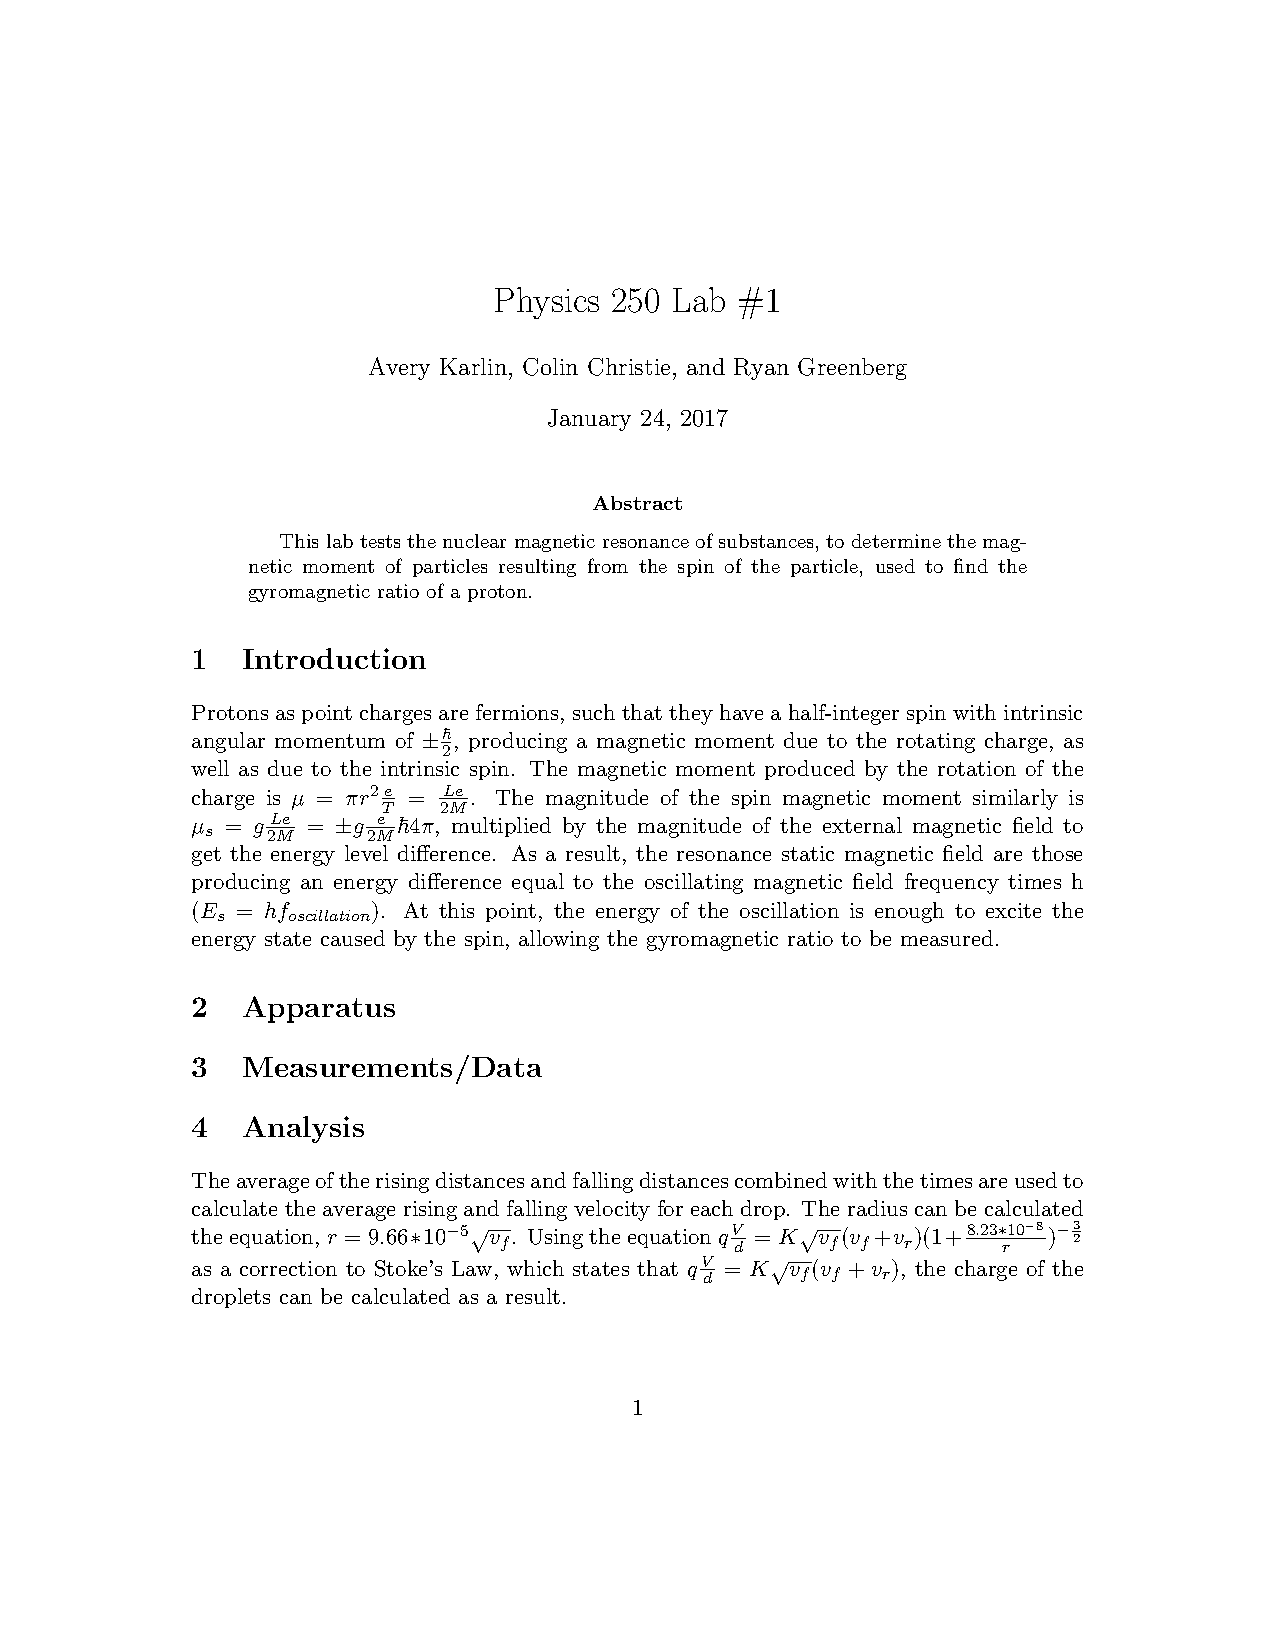
\includegraphics[scale=0.4]{lab8.jpg}
\caption{This is the photo of the setup of the Helmholtz coil to measure the static field produced by the coil with respect to current.}
\label{equip}
\end{center}
\end{figure}

\section{Measurements/Data} \label{Measurements}

\begin{table}[htp]
\begin{center}
\begin{tabular}{|c|c|c|c|}
\hline
Frequency Setting & Period & Frequency & Current 1 & Current 2\\ \hline
1 & 4 $\mu$s & $2.5 * 10^5 s^{-1}$ & 2.62 A & 2.73 A \\
\hline
2 & 5.5 $\mu$s & $1.8 * 10^5 s^{-1}$ & 3.01 A & 3.06 A \\
\hline
3 & 6.75 $\mu$s & $1.48 * 10^5 s^{-1}$ & 3.77 A & 3.74 A \\
\hline
4 & 7.6 $\mu$s & $1.32 * 10^5 s^{-1}$ & 5.14 A & 5.21 A \\
\hline
\end{tabular}
\caption{Measured Data}
\end{center}
\label{table}
\end{table}

It was also found that the inner diameter of the coil is 19.20 cm, while the outer diameter is 22.15 cm, such that the average diameter is 20.675 cm. The outer separation of the 2 loops is 13 cm, while the inner separation is 8.09 cm, such that the average separation is 10.545 cm. It is also measured that the magnetic field in the center of the two loops is -2.26 mT, getting weaker as moving outward radially, unaffected longitudinally. The number of coils on the Helmholtz coil is 12 on one loop, 13 on the other loop. The oscillating component of the magnetic field was found to have a period of 31.8 s, frequency of 0.314 Hz, and amplitude of 0.725 mT.

\section{Analysis and Conclusions}

1. For nuclear magnetic resonance to occur, there must be a nonzero total atomic spin, found in Hydrogen due to the unfilled valence electron shell, causing an electron total spin of one half. Since Helium has a filled valence shell, such that there is a total spin of 0, there is no NMR, while for deuterium, it is still able to occur, due to the spin of the nucleus being integral, the spin of the electrons being half-integral. This is extended to being true that any fermion is able to have NMR. The nucleus is zero spin for those with equal numbers of protons and neutrons, such that He4, Ne20, Ar36, Be8, Mg24, and Ca40 are unable. All others should be able to experience NMR, due to having nonzero spins.

2. It is found by the value of the measurements that g is 0.0349, rather than the expected 1 such that spin doesn’t affect the magnetic moment the same amount as classical orbital electron angular momentum. Protons are expected to have a higher value, such that it implies that they are creating magnetic moments by a different mechanism than electrons, or in a different manner. The significance of the value being a non-whole number is due to the fine-structure refinements.

3. By the formula for $B_h$, it is found that the magnetic field at 5 A is 5.15E-4 T, such that the frequency is 14.44 MHz, such that it is a radio wave.

4. Since the oscillator is required to move the magnetic field over the resonance strength, rather than having to precisely hit the strength, if there was not an oscillator, it would have to be precisely hit by manually varying the signal, which would be vastly harder.

5. The MRI machine is used by finding the resonance of the magnetic field, such that as water is moved within the machine, or some other desired material with a different resonance, the energy is suddenly drastically lost at that particular point, giving the locations of the desired material.

6. The Helmholtz coil arrangement produced a magnetic field either parallel or antiparallel from that of the Earth, such that it had to be taken from both, to determine the effect of a change in the magnetic field of $2B_e$. An additional Helmholtz coil exactly cancelling out that of the Earth could be used instead, or electromagnetic shielding to block the field of the Earth.

7. For each frequency, the time-base is viewed as a sinusoidal curve, based on the direction of electron flow within the wires shifting, causing the electrons to hit different portions of the oscilloscope detector as the force acting on them is distinct.

8. Protons do have an electric dipole, while electrons do not, due to the former being able to be broken up into the composite particles, while a dipole would imply the electron was made up of composite particles. This is not true for a magnetic dipole, due to the lack of existence of magnetic monopoles.

%\end{twocolumn}
\end{document}  